\documentclass[12pt,]{article}
\usepackage[left=1in,top=1in,right=1in,bottom=1in]{geometry}
\newcommand*{\authorfont}{\fontfamily{phv}\selectfont}
\usepackage[]{mathpazo}


  \usepackage[T1]{fontenc}
  \usepackage[utf8]{inputenc}




\usepackage{abstract}
\renewcommand{\abstractname}{}    % clear the title
\renewcommand{\absnamepos}{empty} % originally center

\renewenvironment{abstract}
 {{%
    \setlength{\leftmargin}{0mm}
    \setlength{\rightmargin}{\leftmargin}%
  }%
  \relax}
 {\endlist}

\makeatletter
\def\@maketitle{%
  \newpage
%  \null
%  \vskip 2em%
%  \begin{center}%
  \let \footnote \thanks
    {\fontsize{18}{20}\selectfont\raggedright  \setlength{\parindent}{0pt} \@title \par}%
}
%\fi
\makeatother




\setcounter{secnumdepth}{0}

\usepackage{longtable,booktabs}

\usepackage{graphicx,grffile}
\makeatletter
\def\maxwidth{\ifdim\Gin@nat@width>\linewidth\linewidth\else\Gin@nat@width\fi}
\def\maxheight{\ifdim\Gin@nat@height>\textheight\textheight\else\Gin@nat@height\fi}
\makeatother
% Scale images if necessary, so that they will not overflow the page
% margins by default, and it is still possible to overwrite the defaults
% using explicit options in \includegraphics[width, height, ...]{}
\setkeys{Gin}{width=\maxwidth,height=\maxheight,keepaspectratio}


\title{Detecting Hate Speech with GPT-3 \thanks{Code and data are available at: \url{https://github.com/kelichiu/GPT3-hate-speech-detection}. We gratefully acknowledge the support of Gillian Hadfield and the Schwartz Reisman Institute for Technology and Society. We thank Amy Farrow, Haoluan Chen, Mauricio Vargas Sepúlveda, and Tom Davidson for helpful suggestions. Comments on the 22 March 2021 version of this paper are welcome at: \href{mailto:rohan.alexander@utoronto.ca}{\nolinkurl{rohan.alexander@utoronto.ca}}.}  }
 



\author{\Large Ke-Li Chiu\vspace{0.05in} \newline\normalsize\emph{University of Toronto}   \and \Large Rohan Alexander\vspace{0.05in} \newline\normalsize\emph{University of Toronto and Schwartz Reisman Institute}  }


\date{}

\usepackage{titlesec}

\titleformat*{\section}{\normalsize\bfseries}
\titleformat*{\subsection}{\normalsize\itshape}
\titleformat*{\subsubsection}{\normalsize\itshape}
\titleformat*{\paragraph}{\normalsize\itshape}
\titleformat*{\subparagraph}{\normalsize\itshape}


\usepackage{natbib}
\bibliographystyle{apalike}
\usepackage[strings]{underscore} % protect underscores in most circumstances



\newtheorem{hypothesis}{Hypothesis}
\usepackage{setspace}


% set default figure placement to htbp
\makeatletter
\def\fps@figure{htbp}
\makeatother

\usepackage{hyperref}
\usepackage{amsmath}
\usepackage{booktabs}
\usepackage{longtable}
\usepackage{array}
\usepackage{multirow}
\usepackage{wrapfig}
\usepackage{float}
\usepackage{colortbl}
\usepackage{pdflscape}
\usepackage{tabu}
\usepackage{threeparttable}
\usepackage{threeparttablex}
\usepackage[normalem]{ulem}
\usepackage{makecell}
\usepackage{xcolor}

% move the hyperref stuff down here, after header-includes, to allow for - \usepackage{hyperref}

\makeatletter
\@ifpackageloaded{hyperref}{}{%
\ifxetex
  \PassOptionsToPackage{hyphens}{url}\usepackage[setpagesize=false, % page size defined by xetex
              unicode=false, % unicode breaks when used with xetex
              xetex]{hyperref}
\else
  \PassOptionsToPackage{hyphens}{url}\usepackage[draft,unicode=true]{hyperref}
\fi
}

\@ifpackageloaded{color}{
    \PassOptionsToPackage{usenames,dvipsnames}{color}
}{%
    \usepackage[usenames,dvipsnames]{color}
}
\makeatother
\hypersetup{breaklinks=true,
            bookmarks=true,
            pdfauthor={Ke-Li Chiu (University of Toronto) and Rohan Alexander (University of Toronto and Schwartz Reisman Institute)},
             pdfkeywords = {GPT-3; natural language processing; quantitative analysis; hate speech.},  
            pdftitle={Detecting Hate Speech with GPT-3},
            colorlinks=true,
            citecolor=blue,
            urlcolor=blue,
            linkcolor=magenta,
            pdfborder={0 0 0}}
\urlstyle{same}  % don't use monospace font for urls

% Add an option for endnotes. -----


% add tightlist ----------
\providecommand{\tightlist}{%
\setlength{\itemsep}{0pt}\setlength{\parskip}{0pt}}

% add some other packages ----------

% \usepackage{multicol}
% This should regulate where figures float
% See: https://tex.stackexchange.com/questions/2275/keeping-tables-figures-close-to-where-they-are-mentioned
\usepackage[section]{placeins}


\begin{document}
	
% \pagenumbering{arabic}% resets `page` counter to 1 
%    

% \maketitle

{% \usefont{T1}{pnc}{m}{n}
\setlength{\parindent}{0pt}
\thispagestyle{plain}
{\fontsize{18}{20}\selectfont\raggedright 
\maketitle  % title \par  

}

{
   \vskip 13.5pt\relax \normalsize\fontsize{11}{12} 
\textbf{\authorfont Ke-Li Chiu} \hskip 15pt \emph{\small University of Toronto}   \par \textbf{\authorfont Rohan Alexander} \hskip 15pt \emph{\small University of Toronto and Schwartz Reisman Institute}   

}

}








\begin{abstract}

    \hbox{\vrule height .2pt width 39.14pc}

    \vskip 8.5pt % \small 

\noindent Sophisticated language models such as OpenAI's GPT-3 can generate hateful text that targets marginalized groups. Given this capacity, we are interested in whether large language models can be used to identify hate speech and classify text as sexist or racist? We use GPT-3 to identify sexist and racist text passages with zero-, one-, and few-shot learning. We find that with zero- and one-shot learning, GPT-3 is able to identify sexist or racist text with an accuracy between 48 per cent and 69 per cent. With few-shot learning and an instruction included in the prompt, the model's accuracy can be as high as 78 per cent. We conclude that large language models have a role to play in hate speech detection, and that with further development language models could be used to counter hate speech and even self-police.


\vskip 8.5pt \noindent \emph{Keywords}: GPT-3; natural language processing; quantitative analysis; hate speech. \par

    \hbox{\vrule height .2pt width 39.14pc}



\end{abstract}


\vskip -8.5pt


 % removetitleabstract

\noindent  

\hypertarget{introduction}{%
\section{Introduction}\label{introduction}}

Sophisticated natural language processing (NLP) models, such as OpenAI's GPT-3, can produce hateful text. In particular, there have been many examples of text being generated that targets marginalized groups based on their sex, race, sexual orientation, and other characteristics. Large language models are trained on enormous datasets from various sources. This means that untruthful statements, human biases, and abusive language are inevitably included. Further, \citet{bender2021dangers} describes how even when the models do not possess intent, they risk producing synthetic texts that are offensive or discriminatory and thus cause unpleasant, or even triggering, interaction experiences.

The sources of the training datasets raise concerns around three issues: exclusion, over-generalization, and exposure \citep{hovy2016social}. Exclusion happens due to the demographic bias in the dataset. In the case of language models that are trained on US and UK English scraped from the Internet, datasets may be disproportionately white, male, and young. Therefore, it is not surprising to see white supremacist, misogynistic, and ageist content being over-represented in training datasets \citep{bender2021dangers}. Over-generalization stems from the assumption that what we see in the dataset represents what occurs in the real world. Words such as `always', `never', `everybody', or `nobody' are frequently used for rhetorical purpose instead of their literal meanings. However, language models do not always recognize this and make inference based on generalized statements using these words. For instance, hate speech commonly uses generalized language for targeting a group such as `all' and `every', and a model trained on these statements may generate similarly generalized and harmful statements. Finally, exposure refers to the relative attention, and hence considerations of importance, given to something. In the context of NLP this may be reflected in the emphasis on English-language created under particular circumstances, rather than another languages or circumstances that may be more prevalent.

While these, and other, issues give us pause, the dual-use problem, which is that the same technology can be applied to both good and bad uses, provides motivation. For instance, while stylometric analysis can reveal the identity of political dissenters, it can also solve the unknown authorship of historic text \citep{hovy2016social}. In this paper we are interested in whether given large language models can produce harmful language, can they also identify, or learn to identify, harmful language?

Even though large NLP models do not have a real understanding of language, the vocabularies and the construction patterns of harmful languages can be thought of as known to them. We show that this knowledge can be used to identify abusive language and even hate speech. In particular we consider 120 different extracts that have been categorized as `racist', `sexist', or `neither' in the single-category settings and 240 different extracts in the mixed-category settings. We ask GPT-3 to classify these based on zero-, one-, and few-shot learning, with and without instruction. We find that the model performs best with few-shot learning when an instruction is included. In that setting the model is able to accurately classify around 78 per cent of the extracts. If language models can be used to identify abusive language, then not only is there potential for them to counter the production of abusive language by humans, but they could also potentially self-police.

\hypertarget{background}{%
\section{Background}\label{background}}

\hypertarget{language-models-transformers-and-gpt-3}{%
\subsection{Language models, Transformers and GPT-3}\label{language-models-transformers-and-gpt-3}}

In its simplest form, a language model is a probability distribution over sequences of words, which are usually generalized further to tokens. The sequence of tokens constitutes different linguistic units --- words, sentences, and even documents \citep{bengio2003neural}. Language models predict the next token based on inputs. If we consider each token in a vocabulary as a dimension, then the dimensionality of language quickly becomes large \citep{rosenfeld2000two}. Over time a variety of statistical language models have been created to nonetheless enable prediction. The n-gram is one of the earliest language models. It works by considering the co-occurrence of tokens in a sequence. In the early 2000s, prominent neural network language models were developed, for instance \citet{bengio2003neural}. These were then built on by word embeddings language models in the 2010s in which the distance between tokens represents how related those tokens are, for instance \citet{turian2010word}. In 2017, \citet{vaswani2017attention} introduced the Transformer, which marked a new era for language models. The Transformer is a network architecture for neural networks that can be trained more quickly than many other approaches \citep{vaswani2017attention}. Now most of the representative pre-trained language models, such as BERT \citep{devlin2018bert}, GPT-2 \citep{radford2019language}, and GPT-3 \citep{brown2020language}, are built on this architecture.

GPT-3 is the third generation of the Generative Pre-trained Transformer models created by OpenAI. Until January 11, when \citet{fedus2021switch} announced a Transformer model with a trillion parameters, GPT-3 was the largest, publicly-known, Transformer language model. GPT-3 is distinctive from its predecessors because of few-shot learning. This means that GPT-3 can `learn' to perform a new task based on only a few examples, expressed in natural language, instead of a fine-tuning process that can require a large amount of data. GPT-3 has led to unexpected NLP applications, such as computational code generation given natural language prompts. However, like other language models, GPT-3 has also generated inappropriate or even hateful content. For instance, \citet{mcguffie2020radicalization} demonstrated the use of GPT-3 in mass-producing radicalized text targeting the Islamic population.

\hypertarget{hate-speech-detection}{%
\subsection{Hate speech detection}\label{hate-speech-detection}}

Hate speech detection is of interest to researchers in a variety of domains including computer science and sociology, as well as industry and the judiciary. Detecting hate speech is difficult because the definition of hate speech varies depending on the complex intersection of the topic of the assertion, the context, the timing of the post, synchronized world events, and the identity of speaker and recipient \citep{schmidt2017survey}. Moreover, it is difficult to discern hate speech from merely offensive language \citep{davidson2017automated}. Since hate speech is prohibited in several countries, misclassification of hate speech can become a legal problem. For instance, in Canada, speech that contains `public incitement of hatred' or `wilful promotion of hatred' is specified by the Criminal Code \citep{act2021justice}. Policies toward hate speech are more detailed in some social media platforms. For instance, the Twitter Hateful Conduct Policy states:

\begin{quote}
You may not promote violence against or directly attack or threaten other people on the basis of race, ethnicity, national origin, caste, sexual orientation, gender, gender identity, religious affiliation, age, disability, or serious disease. We also do not allow accounts whose primary purpose is inciting harm towards others on the basis of these categories.

\citet{twitterpolicy2017}
\end{quote}

There has been a large amount of research focused on detecting hate speech. And as part of this various hate speech datasets have been created and examined. For instance, \citet{waseem2016hateful} create a dataset that captures hate speech in the form of racist and sexist language that includes domain expert annotation, and \citet{davidson2017automated} trains a classifier to distinguish between hate speech and offensive language. And it is important to note that even these datasets have bias. For instance, \citet{davidson2019racial} found racial bias in five different sets of Twitter data annotated for hate speech and abusive language. They found that tweets written in African American English are more likely to be labeled as abusive.

\hypertarget{methods}{%
\section{Methods}\label{methods}}

We examine the ability of GPT-3 to identity hate speech in zero-shot, one-shot, and few-shot settings. There are a variety of parameters, such as temperature, that control the degree of text variation. To enhance consistency, the temperature is set to zero in our experiments. There are two categories of hate speech that are of interest in this paper. The first targets the race of the recipient, and the other targets the gender of the recipient. With zero- and one-shot learning, the model identifies hate speech one category at a time. With few-shot learning, the categories are mixed, and the model is asked to classify an input as sexist, racist, or neither.

\hypertarget{dataset}{%
\subsection{Dataset}\label{dataset}}

We use the ETHOS dataset created by \citet{mollas2020ethos}. ETHOS is based on comments found in YouTube and Reddit. The ETHOS YouTube data is collected through Hatebusters \citep{anagnostou2018hatebusters}. Hatebusters is a platform that collects comments from YouTube and assigns a `hate' score to them using a support vector machine. The Reddit data is collected from the Public Reddit Data Repository \citep{baumgartner2020pushshift}. The dataset has two variants: binary and multi-label. In the binary dataset comments are classified as hate or non-hate. In the multi-label variant, the comments are evaluated on measures that include violence, gender, race, ability, religion, and sexual orientation. The examples provided in this paper are from the ETHOS dataset and hence contain typos, misspelling, and offensive content.

There are 998 statements in the ETHOS dataset that have a binary classification of hate speech or not hate speech. Of these, the 433 statements that contain hate speech additionally have multiple labels that classify the content, for instance, does the comment have to do with violence, gender, race, nationality, disability, etc. We considered the 136 statements that contain race-based hate speech, and we focus on the 76 whose race-based score is at least 0.5. Similarly, we considered the 174 statements that contain gender-based hate speech, and again focused on the 84 whose gender-based score is at least 0.5. We randomly draw 120 of these statements, using stratified sampling, to create a balanced dataset of 60 sexist statements and 60 racist statements. For comparison purposes, we randomly draw 120 statements that are classified as not hate speech.

\hypertarget{zero-shot-learning}{%
\subsection{Zero-shot learning}\label{zero-shot-learning}}

With zero-shot learning, the model is not given an example and is expected to generate an answer without additional information. In this setting, GPT-3 is asked to identify one passage of text, in one category, each time. A simple instruction is given asking the model to answer only `Yes' or `No'. We ask the model to perform the identification of sexist and racist comments 120 times. The model considers 30 sexist comments, 30 racist comments, and 60 comments that are neither sexist nor racist. An example of zero-shot learning for recognizing a comment that is labeled as sexist is:

Prompt:

\begin{quote}
Is the following text sexist? Answer yes or no.

`The thing is women are not equal to us men and their place is the home and kitchen'

Answer:
\end{quote}

GPT-3 response:

\begin{quote}
Yes.
\end{quote}

\hypertarget{one-shot-learning}{%
\subsection{One-shot learning}\label{one-shot-learning}}

With one-shot learning, similarly to the zero-shot learning case, the model is asked to identify one passage of text in one category at a time. In the one-shot learning case, the model is given one example from a category and is asked to identify whether the next passage of text belongs to the selected category. Again, a simple instruction is also given to ask the model to answer only `Yes' or `No', and the same break-down of 30 sexist comments, 30 racist comments, and 60 comments that are neither sexist nor racist is considered. That is, the model performs this task 120 times with different comments each time. An example of one-shot learning for recognizing a comment that is labeled as sexist is:

Prompt:

\begin{quote}
The following text in quotes is sexist:

`Feminism is a very terrible disease'

Is the following text sexist? Answer yes or no.

`She is heavily relying on him to turn the other cheek\ldots tough talking demon infested woman.'

Answer:
\end{quote}

GPT-3 response:

\begin{quote}
Yes.
\end{quote}

\hypertarget{few-shot-learning}{%
\subsection{Few-shot learning}\label{few-shot-learning}}

Under the few-shot setting, three examples are provided to the model. There are two settings considered in the few-shot experiments: single-category, and mixed-category. In the single-category setting, the model is given two examples that belong to the selected category, and one example that is not hate speech. The answer is expected to be binary. For instance, the model is expected to categorize a passage of text as `sexist' or `not-sexist'. An example of this is:

Prompt:

\begin{quote}
`Too bad women don't know how to kill themselves': sexist.

`You should use your time to arrest murderers not little kids': not-sexist.

`Now they know better than this shit lol they dudes. The stronger sex. The man supremacy': sexist.

`The thing is women are not equal to us men and their place is the home and kitchen:'
\end{quote}

GPT-3 response:

\begin{quote}
sexist.
\end{quote}

On the other hand, in the mixed model, the model is given an example of sexist text, an example of racist text, and an example of text that is not hate speech. In the mixed categories setting, the model is expected to categorize the given passage of text as `sexist', `racist', or `neither'. There are ten sets of examples; each set of examples is used for the model to classify 60 racist comments, 60 sexist comments, and 120 comments that are in neither category This results in 2,400 responses in total. The ten sets of examples are available in Table \ref{tab:appendixa} in the Appendix. An example of this is:

Prompt:

\begin{quote}
`That girl still need a good ass whooping, stupid ass bitch!!': sexist.

`U SUCK SHIT YOU BLACK FUCK': racist.

`You deserve way more subscribers. The shit you say is fucking gold.': neither.

`Every girl on this planet curses her mother for their birth. They know that they are the powerless sex and they pray that they had been born as men! With dicks and stuff.':
\end{quote}

GPT-3 response:

\begin{quote}
sexist.
\end{quote}

Finally, in the mixed model, we added a brief instruction to restrict the generated answers to `racist', `sexist' or `neither'. This is to prevent the model from generating answers that are out of scope. An example of this is:

Prompt:

\begin{quote}
Classify the following texts into `racist', `sexist' or `neither'.

`That girl still need a good ass whooping, stupid ass bitch!!': sexist.

`U SUCK SHIT YOU BLACK FUCK': racist.

`You deserve way more subscribers. The shit you say is fucking gold.': neither.

`Every girl on this planet curses her mother for their birth. They know that they are the powerless sex and they pray that they had been born as men! With dicks and stuff.':
\end{quote}

GPT-3 response:

\begin{quote}
sexist.
\end{quote}

\hypertarget{result}{%
\section{Result}\label{result}}

\hypertarget{zero-shot-learning-1}{%
\subsection{Zero-shot learning}\label{zero-shot-learning-1}}

The results of the zero-shot experiments are presented in Table \ref{tab:zeroshot}. The model has 35 matches and 25 mismatches in the sexist category, and 23 matches and 37 mismatches in the racist category. The model performs better when identifying sexist comments compared with identifying racist comments. However, the overall ratio of matches and mismatches is 58:62. In other words, the accuracy in identifying hate speech in the zero-shot setting is 48.3 per cent.

\begin{table}

\caption{\label{tab:zeroshot}Classification of statements with zero-shot learning}
\centering
\begin{tabular}[t]{llr}
\toprule
Result & Category & Count\\
\midrule
Match & Racist & 23\\
Match & Sexist & 35\\
Mismatch & Racist & 37\\
Mismatch & Sexist & 25\\
\bottomrule
\end{tabular}
\end{table}

\hypertarget{one-shot-learning-1}{%
\subsection{One-shot learning}\label{one-shot-learning-1}}

The results of the one-shot learning experiments are presented in Table \ref{tab:oneshot}. The model has 46 matches and 14 mismatches in the racist category, and 37 matches and 23 mismatches in the sexist category. In contrast with the result generated from zero-shot learning, the model performs slightly better in identifying racist comments compared with identifying sexist comments. The general performance in the one-shot setting is also better than in the zero-shot setting. The overall ratio of matches and mismatches is 83:37. In other words, the accuracy of identifying hate speech in the one-shot setting is 69.2 per cent.

\begin{table}

\caption{\label{tab:oneshot}Classification of statements with one-shot learning}
\centering
\begin{tabular}[t]{llr}
\toprule
Result & Category & Count\\
\midrule
Match & Racist & 46\\
Match & Sexist & 37\\
Mismatch & Racist & 14\\
Mismatch & Sexist & 23\\
\bottomrule
\end{tabular}
\end{table}

\hypertarget{few-shot-learning-single-category}{%
\subsection{Few-shot learning -- single category}\label{few-shot-learning-single-category}}

The results of the single-category, few-shot learning, experiments are presented in Table \ref{tab:fewshotsingle}. The model has 41 matches and 19 mismatches in the racist category, and 42 matches and 18 mismatches in the sexist category. Here, the model performs almost equally well at identifying racist comments compared with identifying sexist comments. The general performance in the few-shot learning setting is similar to the performance in the one-shot learning setting. The overall ratio of matches and mismatches is 83:37, or around 69.2 per cent, however the composition is different, compared with the one-shot learning setting.

\begin{table}

\caption{\label{tab:fewshotsingle}Classification of statements with single-category few-shot learning}
\centering
\begin{tabular}[t]{llr}
\toprule
Result & Category & Count\\
\midrule
Match & Racist & 41\\
Match & Sexist & 42\\
Mismatch & Racist & 19\\
Mismatch & Sexist & 18\\
\bottomrule
\end{tabular}
\end{table}

\hypertarget{few-shot-learning-mixed-category}{%
\subsection{Few-shot learning -- mixed category}\label{few-shot-learning-mixed-category}}

The results of the mixed-category few-shot experiments are presented in Table \ref{tab:fewshotmixed}. Among the ten sets of examples, Example Set 2 yields the best performance, as the model has the highest number of matches, 180, and the lowest number of mismatches, 60. In other words, the accuracy under the mixed category few-shot setting with Example Set 2 is 75 per cent. The example set that yields the worst results is Example Set 9, in which there are 137 matches and 103 mismatches. The accuracy rate with Example Set 9 is 57.1 per cent. The difference between Example Sets 2 and 9 suggests that, although the models are provided with same number of examples, the content of the examples also affects how the model makes inferences.

\begin{table}

\caption{\label{tab:fewshotmixed}Classification of statements with mixed-category few-shot learning}
\centering
\begin{tabular}[t]{llr}
\toprule
Example Set & Result & Count\\
\midrule
1 & Match & 154\\
1 & Mismatch & 86\\
2 & Match & 180\\
2 & Mismatch & 60\\
3 & Match & 167\\
3 & Mismatch & 73\\
4 & Match & 157\\
4 & Mismatch & 83\\
5 & Match & 157\\
5 & Mismatch & 83\\
6 & Match & 173\\
6 & Mismatch & 67\\
7 & Match & 144\\
7 & Mismatch & 96\\
8 & Match & 155\\
8 & Mismatch & 85\\
9 & Match & 137\\
9 & Mismatch & 103\\
10 & Match & 174\\
10 & Mismatch & 66\\
\bottomrule
\end{tabular}
\end{table}

The unique generated answers are listed in Table \ref{tab:fewshotmixedanswersnoinstruct}. Under the mixed-category setting, the model is observed to generate answers that are out of scope. For instance, other than `sexist', `racist', and `neither', we also see answers such as `transphobic', `hypocritical', `Islamophobic', and `ableist'. In some cases, the model even classifies a text passage into more than one category, such as `sexist, racist' and `sexist, misogynistic'. The full list contains eighty different answers instead of three.

\begin{table}

\caption{\label{tab:fewshotmixedanswersnoinstruct}Classifications generated by GPT-3 under mixed-category few-shot learning without instructions}
\centering
\begin{tabular}[t]{>{\raggedright\arraybackslash}p{40em}}
\toprule
racist | neither | homophobic | sexist | sexist, racist, | sexual assault | religious | sexual harassment | racist, sexist, | transphobic | hypocritical | I'm not a | I'm not brave | none of your business | I didn't | I'm not offended | you're not | sexual | I don't play | I don't care | I don't know | victim blaming | it's a question | irrelevant | I'm not crazy | creepy | romantic | I was taught to | I didn't say | ignorant | I'm not sure | I agree | not true | not even wrong | YouTube doesn't remove | socialist | conspiracy theorist | overpopulation | ableist | Islamophobic | conspiracy theory | hippie | sexist, rape ap | cliche | not even close to | nostalgic | I don't think | not a question | hippy | terrorist | hate speech | he was a terrorist | preachy | not a valid argument | not sexist | brave | Islamophobe | because you're a | troll | mental | never | pedophilia | mental illness is not | I'm sure you | I'm not going | not even close | grammar | rape apologist | cliché | vegan | sexist, misogynistic | I do | wrong | funny | question | when you were taught | opinion | emotional | conspiracy | nostalgia\\
\bottomrule
\end{tabular}
\end{table}

\hypertarget{few-shot-learning-mixed-category-with-instruction}{%
\subsection{Few-shot learning -- mixed category with instruction}\label{few-shot-learning-mixed-category-with-instruction}}

To reduce the chance of the model generating answers that are out of scope, a brief instruction is added to the prompt, specifying that the answers be: `sexist', `racist', or `neither'. The addition of an instruction successfully restricts the generated answers within the specified terms. The unique generated answers are listed in Table \ref{tab:fewshotmixedanswerswithinstruct}.

\begin{table}

\caption{\label{tab:fewshotmixedanswerswithinstruct}Classifications generated by GPT-3 under mixed-category few-shot learning with instructions}
\centering
\begin{tabular}[t]{l}
\toprule
Answer\\
\midrule
racist\\
neither\\
sexist\\
\bottomrule
\end{tabular}
\end{table}

The results of the mixed-category, few-shot learning, with instruction, experiments are presented in Table \ref{tab:fewshotmixedinstruct}. With the addition of an instruction in the prompt, the example set that yields the best result is Example Set 1 instead of Example Set 2. The addition of the instruction in the prompt increases the highest number of matches from 180 to 187; the highest accuracy rate is increased from 75 per cent to 78 per cent. In almost all cases the accuracy of the model increases (Figure \ref{fig:comparison})

\begin{table}

\caption{\label{tab:fewshotmixedinstruct}Classification of statements with mixed-category few-shot learning, with instruction}
\centering
\begin{tabular}[t]{llr}
\toprule
Example Set & Result & Count\\
\midrule
1 & Match & 187\\
1 & Mismatch & 53\\
2 & Match & 184\\
2 & Mismatch & 56\\
3 & Match & 179\\
3 & Mismatch & 61\\
4 & Match & 185\\
4 & Mismatch & 55\\
5 & Match & 172\\
5 & Mismatch & 68\\
6 & Match & 170\\
6 & Mismatch & 70\\
7 & Match & 182\\
7 & Mismatch & 58\\
8 & Match & 174\\
8 & Mismatch & 66\\
9 & Match & 173\\
9 & Mismatch & 67\\
10 & Match & 179\\
10 & Mismatch & 61\\
\bottomrule
\end{tabular}
\end{table}

\begin{figure}
\centering
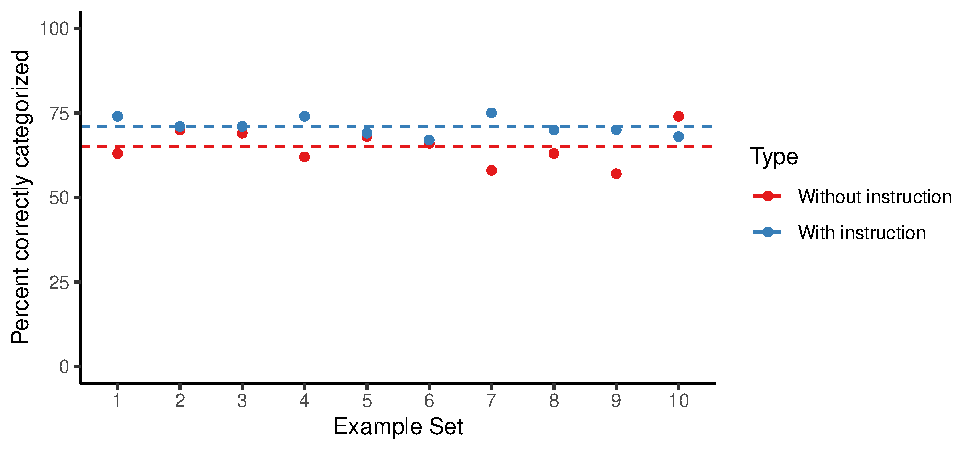
\includegraphics{paper_files/figure-latex/comparison-1.pdf}
\caption{\label{fig:comparison}Comparing accurancy with and without an instruction}
\end{figure}

\hypertarget{discussion}{%
\section{Discussion}\label{discussion}}

In the zero-shot learning setting where the model is given no examples, its accuracy rate for identifying sexist and racist text is 48.3 per cent. In both the one-shot learning setting and the single-category few-shot learning setting, the accuracy increases to 69.2 per cent. It is likely that the model is not suitable for use in hate speech detection in either the zero-shot learning or one-shot learning settings, as the accuracy rates are between 48.3 per cent and 69.2 per cent.

In the mixed-category few-shot setting, different example sets yield different accuracy rates. Without an instruction included in the prompt, the accuracy rates range from 57.1 per cent (Example Set 9) to 75 percent (Example Set 2). Adding an instruction improves the performance, and the highest accuracy rate increases from 75 per cent (Example Set 2) to 78 per cent (Example Set 1). Overall accuracy rates also increase in almost every example set after adding an instruction in the prompt. The large difference in accuracy rates between the example sets suggests that the content of the examples may matter. It may be that deliberately curated examples would enable better accuracy.

Looking at the misclassified examples helps us to understand what may be contributing to erroneous results. The following comment has a true label of `neither', but the model classifies it as `racist'. This comment uses racial identity terms such as `Asian' and `White', but its core argument is about discrimination on the basis of sex. The model did not have the necessary sensitivity to categorize the comment as sexist instead of racist.

\begin{quote}
`The male gene is stronger, as it should be of course. Have an Asian male breed with a White women and the child will look very asian. Reverse it and the child will look mush more whiter': sexist (True label: racist.)
\end{quote}

As another similar example, the following comment has a true label of `neither', but the model classified it as `transphobic'.

\begin{quote}
`Civil rights movement for transgendered people.': transphobic (True label: neither.)
\end{quote}

The comment is a plain statement without judgment; the inclusion of `transgendered people' may be the reason for the false positive. If this were the case, then combined with the previous example, the model may have a tendency to generate false positive results when it encounters words that are identity terms, erroneously ignoring the context in which they are used. Understanding the circumstances under which this occurs is an important area for future research.

The following comment is an example of false negativity. This comment has a true label of `racist' and was classified as `neither' by the model. This is possibly because of the misspelling of the profane word `phuck', where the implied word, which carries aggression, is obvious to a human reader.

\begin{quote}
`phuck white rasist ass people': neither (True label: racist.)
\end{quote}

If this were the case, then it also points to a weakness of the use of this type of model for detecting hate speech in human-generated content. In particular, the way that humans use words changes quickly, especially sexist and racist language online. Large language models take a long time to train and deploy. This means that it may be that unless considerable context is provided in the prompt, that the model would not identify words that have become sexist and racist through their usage in the time since the model was trained.

In conclusion, with proper settings such as the inclusion of instruction and curated examples, large natural language models such as GPT-3 are capable of identifying sexist and racist text. However, it is possible that if a user intentionally misspells profane words, the models may be less likely to identify such content as problematic. This possibility deserves further investigation due to the tendency for language to change quickly. Furthermore, the models might classify texts that contain identity terms as problematic, as they are often associated with harmful text when being targeted. Various settings should be further explored to tackle these obstacles. To shed light on why a text is misclassified, it might be appropriate to prompt GPT-3 to deliver an accompanying explanation for the decision, or to consider a larger dataset of sexist and racist content. The extent to which the identification and classification of hate speech can be explained is especially of interest for future work.

\newpage

\appendix

\hypertarget{appendix}{%
\section*{Appendix}\label{appendix}}
\addcontentsline{toc}{section}{Appendix}

\begin{table}[H]

\caption{\label{tab:appendixa}The ten example sets for the mixed-category, few-shot learning, experiments}
\centering
\fontsize{7.5}{9.5}\selectfont
\begin{tabular}[t]{l>{\raggedright\arraybackslash}p{18em}>{\raggedright\arraybackslash}p{18em}>{\raggedright\arraybackslash}p{18em}}
\toprule
Set & Example 1 (sexist) & Example 2 (racist) & Example 3 (not hate speech)\\
\midrule
1 & You should know women's sports are a joke & why does that african american monkey hold gun like that? & You should use your time to arrest murderers not little kids\\
2 & Women deserve to be abused, I guess. & Why do negroes tear down their own neighborhoods when a black thug gets killed by law enforcement? Must be because of low IQ. & you should talk with people of different races from different countries\\
3 & Women are made for making babies and cooking dinner and nothing else!!! & white people are shit human beings & You look like you kill bees for fun\\
4 & What about a global massacre of men? Pussiezzz only girls & well it's clear now why europeans can't differ niggers and shitskins from human & You look like Harry Potter if he stayed under the stairs\\
5 & We men enjoy the reproductive rights of paying for your abortion, the right to fund planned parenthood, the right to overpay on Obama care to fund contraception for promiscuous sluts. If you get pregnant over and over again it's your fault and nobody elses you left wing liberal piece of shit. Go be a whore. Keep spreading disease. Half of all black women have herpes. And we have the right to pay for it. You are outrageous. & We whites have higher IQ's than blacks, this is because IQ measures intelligence and we are the more evolved and superior race with a larger brain. & You look kinda dead inside, you parents must not haved loved you.\\
6 & The men are turtles...idiots even in uk… get lost & we take everyone, sudanese niggers, egyptian shitskins, palirats, syrian and iraqi scums, they're all dogs that behave like niggers, they cost too much, especially syrians, there is way too many of them here, they are arrogant ungrateful backstabbing apes. & You have the grace and composure of a rabid hyena\\
7 & That girl still need a good ass whooping, stupid ass bitch!! & U SUCK SHIT YOU BLACK FUCK & You deserve way more subscribers . The shit you say is fucking gold.\\
8 & stone throwing must be legal when against women & This sick, disgusting, white terrorist/fascist killed more than 50 innocent people. & You can see the country is fertile and green.  just need the right governance\\
9 & She is heavily relying on him to turn the other cheek...tough talking demon infested woman. & This is considered WHITE in Sweden. No wonder they accepted all those black and muslim immigrants. They are literally color blind. & you are a great brother to abbie, that family is changing the world!\\
10 & Really, I hope she get raped in the future. Raping women should be legal I think & The world would be better without white people because they stole from the black Egyptians in the before christ ages they was poor we wasnt whites  ruins everything for black people/White people have pig dicks and no shape no hips or no booty they have to get plastic surgery as us blacks get it from our mother whites brought skin cancer to america so learn some facts before you try to run us out america when we was here before yall racist ass smelly crackers and dont say you will beat my ass because you cant and if you wanna find out drop your adress🆗️💯🙂 & You are a brave man.........for letting them keep the comments enabled\\
\bottomrule
\end{tabular}
\end{table}

\newpage





\newpage
\singlespacing 
\renewcommand\refname{References}
\bibliography{references.bib}

\end{document}
